\ifx\allfiles\undefined
\documentclass[a4paper]{book}
\usepackage{ctex}
\usepackage{graphicx} %插入图片
\usepackage{amsmath,amsthm}
\usepackage{lmodern}
\usepackage{float}
\usepackage[export]{adjustbox}
\usepackage{listings,xcolor} %代码块
\usepackage{xcolor}
\usepackage{listings}
\lstset{
    breaklines,                                 % 自动将长的代码行换行排版
    extendedchars=false,                        % 解决代码跨页时,章节标题,页眉等汉字不显示的问题
    backgroundcolor=\color[rgb]{0.96,0.96,0.96},% 背景颜色
    keywordstyle=\color{blue}\bfseries,         % 关键字颜色
    identifierstyle=\color{black},              % 普通标识符颜色
    commentstyle=\color[rgb]{0,0.6,0},          % 注释颜色
    stringstyle=\color[rgb]{0.58,0,0.82},       % 字符串颜色
    showstringspaces=false,                     % 不显示字符串内的空格
    numbers=left,                               % 显示行号
    numberstyle=\small\ttfamily,                % 设置数字字体
    basicstyle=\small\ttfamily,                 % 设置基本字体
    captionpos=t,                               % title在上方(在bottom即为b)
    frame=single,                               % 设置代码框形式
    rulecolor=\color[rgb]{0.8,0.8,0.8},         % 设置代码框颜色
}  
   

\begin{document}
\fi

\section{符号}

\begin{gather*}
%     \centering
    a \& (b\mid c) = (a\&b)\mid(a\&c)\\
    a \oplus (b\mid c) = (a\oplus b)\mid(a\oplus c)\\
    a\mid (a\&b) = a\\
    a\&(a\mid b) = a\\
    (a+b) = (a\mid b)+(a\&b)\\
\end{gather*}

\section{快速幂}
\begin{lstlisting}[language=C++]
ll ksm(ll b,ll p)
{
    ll r=1;
    while(p>0)
    {
        if(p&1) r=(r%mod*(b%mod))%mod;
        p>>=1;b=(b%mod*(b%mod))%mod;
    }
    return r;
}
\end{lstlisting}

\section{快速乘}
\begin{lstlisting}[language=C++]
ll ksc(ll a,ll b) 
{
	ll re=0;
	while(b) 
	{
		if(b&1)	re=(re+a)%mod;
		b>>=1;a=(a+a)%mod;
	}
	return re;
}
\end{lstlisting}

\section{组合数学}

\begin{gather*}
    C_{n+1}^{m} = C_{n} ^ {m} + C_{n} ^ {m-1}\\
    C_{n} ^ {0} + C_{n} ^ {1} + C_{n} ^ {2} + ... + C_{n} ^ {n} =2 ^ n\\
    C_{n} ^ {0} + C_{n} ^ {2} + C_{n} ^ {4} +... = C_{n} ^ {1} + C_{n} ^ {3} + C_{n} ^ {5} + ... = 2^{n-1}
\end{gather*}
\subsubsection{不相邻的排列}
$1\sim n$这$n$个自然数中选$k$个,这$k$个数中任何两个数都不相邻的组合有$\binom{n-k+1}{k}$种。
\subsubsection{错位排列}
\indent$n$封不同的信,编号分别是$1,2,3,4,5$ ,现在要把这五封信放在编号$1,2,3,4,5$的信封中,要求信封的编号与信的编号不一样。问有多少种不同的放置方法?\\
\indent$f(n)$为有$n$封信的错排方式,$f(n)=(n-1)(f(n-1)+f(n-2))$。\\
\indent错位排列数列的前几项为$0,1,2,9,44,265$。
\subsubsection{圆排列}
\indent$n$个人围成一个圆,圆的所有组成排列数记为$Q_n^{n}$,其中$Q_n^{n} \times n=A_n^n$。\\
\indent由此可知部分圆排列的公式:
$$
Q_n^r=\frac{A_n^r}{r}=\frac{n!}{r\times(n-r)!}
$$
\section{Lucas定理}
\begin{lstlisting}[language=c++]
ll C(ll n,ll m)
{
    if(n<m) return 0;
    if(m>n-m) m=n-m;
    ll a=1,b=1;
    for(int i=0;i<m;i++)
    {
        a=(a*(n-i))%mod;b=(b*(i+1))%mod;
    }
    return a*ksm(b,mod-2)%mod;
}
ll lucas(ll n,ll m)
{
    if(m==0)  return 1;
    return lucas(n/mod,m/mod)*C(n%mod,m%mod)%mod;
}
\end{lstlisting}
\section{预处理版本组合数}
\begin{lstlisting}[language=c++]
void binom_init(int x) {
    fac[0] = fac[1] = 1;
    inv[1] = 1;
    finv[0] = finv[1] = 1;
    for(int i=2; i<x; i++){
        fac[i] = fac[i-1]*i%mod;
        inv[i] = mod-mod/i*inv[mod%i]%mod;
        finv[i] = finv[i-1]*inv[i]%mod;
    }
}
ll binom(ll n, ll r){
    if(n<r || n<0 || r<0) return 0;
    return fac[n]*finv[r]%mod*finv[n-r]%mod;
}
\end{lstlisting}
\section{线性筛}
\begin{lstlisting}[language=c++,escapeinside=``]
int primes[N],cnt; //`primes[]存储所有素数`
bool st[N]; //`st[x]存储x是否被筛掉`
void get_primes(int n)
{
    for(int i=2;i<=n;i++)
    {
        if(!st[i]) primes[cnt++]=i;
        for (int j=0;primes[j]<=n/i;j++)
        {
            st[primes[j]*i]=true;
            if(i%primes[j]==0) break;
        }
    }
}
\end{lstlisting}
\section{Miller-Rabin素性测试}
\begin{lstlisting}[language=c++,escapeinside=``]
bool millerRabin(int n) 
{
    if(n<3||n%2==0) return n==2;
    int a=n-1,b=0;
    while(a%2==0) a/=2,++b;
    // `test\_time 为测试次数,建议设为不小于8`
    // `的整数以保证正确率,但也不宜过大,否则会影响效率`
    for(int i=1,j;i<=test_time;++i) 
    {
        int x=rand()%(n - 2)+2,v=quickPow(x,a,n);
        if(v==1) continue;
        for(j=0;j<b;++j) 
        {
            if(v==n-1) break;
            v=(long long)v*v%n;
        }
        if(j>=b) return 0;
    }
    return 1;
}
\end{lstlisting}
\section{欧拉函数}
欧拉函数,即$\varphi(n)$,表示的是小于等于$n$和$n$互质的数的个数。比如说$\varphi(1)=1$。当$n$是质数的时候,显然有$\varphi(n)=n-1$。
\begin{lstlisting}[language=c++,escapeinside=``]
void ora(int n)
{
    phi[1]=1;
    for(int i=2;i<=n;i++)
    {
        if(!st[i])  //`i是质数`
        {
            primes[cnt++] = i;
            phi[i] = i-1;
        }
        for(int j=0;primes[j]*i<=n;j++)
        {
            st[i*primes[j]]=true;
            //`情况1 primes[j]是i的最小质因子`
            if(i%primes[j]==0)
            {
                phi[i*primes[j]] = phi[i]*primes[j];
                break;
            }
            //`情况2`
            phi[i*primes[j]] = phi[i]*(primes[j]-1);
        }
    }
}
\end{lstlisting}

\section{线性代数}
\subsection{矩阵}
\subsubsection{矩阵乘法}
\indent设$A$为$P\times M$的矩阵,$B$为$M\times Q$的矩阵,设矩阵$C$为矩阵$A$与$B$的乘积,其中矩阵$C$中的第$i$行第$j$列元素可以表示为:\\
$$
C_{i,j}=\displaystyle\sum_{k=1}^{M}A_{i,k}B_{k,j}
$$
\indent口诀为\textbf{前行乘后列}。\\
\indent矩阵乘法满足结合律,不满足一般的交换律。利用结合律,矩阵乘法可以利用\textbf{快速幂}的思想来优化。\\
\begin{lstlisting}[language=c++,title=使用二维数组模拟矩阵]
struct mat 
{
    ll a[sz][sz];
    inline mat(){memset(a,0,sizeof(a));}
    inline mat operator-(const mat& T) const 
    {
        mat res;
        for(int i=0;i<sz;i++)
            for(int j=0;j<sz;j++) 
                res.a[i][j]=(a[i][j]-T.a[i][j])%mod;
        return res;
    }
    inline mat operator+(const mat& T) const 
    {
        mat res;
        for(int i=0;i<sz;i++)
            for(int j=0;j<sz;j++) 
                res.a[i][j]=(a[i][j]+T.a[i][j])%mod;
        return res;
    }
    inline mat operator*(const mat& T) const 
    {
        mat res;
        int r;
        for(int i=0;i<sz;i++)
            for(int k=0;k<sz;k++) 
            {
                r=a[i][k];
                for(int j=0;j<sz;j++)
                    res.a[i][j]+=T.a[k][j]*r,res.a[i][j]%=mod;
            }
        return res;
    }
    inline mat operator^(ll x) const 
    {
        mat res,bas;
        for(int i=0;i<sz;i++) res.a[i][i]=1;
        for(int i=0;i<sz;i++)
            for(int j=0;j<sz;j++) bas.a[i][j]=a[i][j]%mod;
        while(x) 
        {
            if(x&1) res=res*bas;
            bas=bas*bas;x>>=1;
        }
        return res;
    }
};
\end{lstlisting}
\subsubsection{矩阵加速递推}
矩阵加速的核心是加速矩阵的构造。以斐波那契数列为例,其递推式:\\
$$
F(n)=F(n-1)+F(n-2)
$$
也就是对于$F(n)$来说,对其推导有用的只有$F(n-1)$和$F(n-2)$。我们将他们放在同一个矩阵里。(顺序无所谓)\\
$$
\begin{bmatrix}
    F(n-2)\\F(n-1)
\end{bmatrix} 
$$
考虑我们对这个矩阵不断左乘一个加速矩阵有什么效果。
$$
\begin{bmatrix}
    0 & 1\\1 & 1
\end{bmatrix} \times
\begin{bmatrix}
    F(n-2)\\F(n-1)
\end{bmatrix} =
\begin{bmatrix}
    F(n-1)\\F(n)
\end{bmatrix} 
$$
$$
\begin{bmatrix}
    0 & 1\\1 & 1
\end{bmatrix} \times
\begin{bmatrix}
    F(n-1)\\F(n)
\end{bmatrix} =
\begin{bmatrix}
    F(n)\\F(n+1)
\end{bmatrix} 
$$
$$
\begin{bmatrix}
    0 & 1\\1 & 1
\end{bmatrix} \times
\begin{bmatrix}
    F(n)\\F(n+1)
\end{bmatrix} =
\begin{bmatrix}
    F(n+1)\\F(n+2)
\end{bmatrix}
$$
所以:\\
$$
\begin{bmatrix}
    F(n-1)\\F(n)
\end{bmatrix} =
\begin{bmatrix}
    0 & 1\\1 & 1
\end{bmatrix}^{n-2} \times
\begin{bmatrix}
    F(1)\\F(2)
\end{bmatrix}
$$
矩阵快速幂即可快速求解。
\subsubsection{其他数列的递推方法}
假设我们目标构造$F(n)=F(n-1)+F(n-2)+1$。首先,将对$F(n)$有用的信息放在一个列向量里:
$$
\begin{bmatrix}
    F(n-2)\\F(n-1)\\1
\end{bmatrix}
$$
为其构造$n*n$大小的加速矩阵,该矩阵应为:
$$
\begin{bmatrix}
    0 & 1 & 0\\1 & 1 & 1\\0 & 0 & 1
\end{bmatrix}
$$
\subsubsection{floyed矩阵优化DP}
我们定义floyed矩阵乘法如下:
$$
\begin{bmatrix}1 \quad 1\\1\quad 0\end{bmatrix}*\begin{bmatrix}f[n] \\ f[n-1]\end{bmatrix}=\begin{bmatrix}max\{f[n]+1,f[n-1]+1\} \\ max\{f[n]+1,f[n-1]+0\}\end{bmatrix}
$$

\subsection{线性基}
\begin{lstlisting}[language=c++]
void add(int x)
{
    for(int i=62;i>=0;i--)
    {
        if(x>>i&1)
        {
            if(!p[i])
            {
                p[i]=x;break;
            }
            else x^=p[i];
        }
    }
}
\end{lstlisting}
\subsubsection{性质}
\begin{itemize}
    \item 原序列里面的任意一个数都可以由线性基里面的一些数异或得到。
    \item 线性基里面的任意一些数异或起来都不能得到$0$。
    \item 线性基里面的数的个数唯一,并且在保持性质一的前提下,数的个数是最少的。
\end{itemize}
\subsubsection{证明性质1}
\indent若数字$x$\textbf{不能插入线性基},显然就是它在尝试插入时异或若干个数之后变成了$0$,即$x\oplus p[a] \oplus p[b] \cdots=0$,则有$p[a] \oplus p[b] \cdots=x$,所以,如果$x$不能成功插入线性基,一定是因为当前线性基里面的一些数异或起来可以等于$x$。\\
\indent若数字$x$\textbf{能插入线性基},我们假设$x$插入到了线性基的第$i$个位置,显然,它在插入前可能异或若干个数,那么就有:$p[a] \oplus p[b] \cdots=p[i]$。同理这样的$x$也可以在线性基上找到。
\subsubsection{证明性质2}
若性质$2$可以满足,则有$p[a] \oplus p[b] \oplus \cdots\oplus =p[c]$,那么$p[c]$就不可能会被插入线性基中。结果矛盾,性质无法成立。
\subsubsection{序列异或最大值}
\begin{lstlisting}[language=c++]
ll query_max()
{
    ll anss=0;
    for(int i=60;i>=0;i--)//记得从线性基的最高位开始
        if((anss^p[i])>anss)anss^=p[i];
    return anss;
}    
\end{lstlisting}
\subsubsection{序列异或最小值}
\begin{lstlisting}[language=c++]
ll query_min()
{
    for(int i=0;i<=60;i++)
        if(p[i]) return p[i];
    return 0;
}    
\end{lstlisting}
\subsubsection{序列异或第$k$小}
\begin{lstlisting}[language=c++,escapeinside=``]
void work()//处理线性基
{
    for(int i=1;i<=60;i++)
    for(int j=1;j<=i;j++)
    if(d[i]&(1ll<<(j-1)))d[i]^=d[j-1];
}
ll k_th(ll k)
{
    //`假如k=1,且原来的序列可以异或出0,返回0。tot表示线性基中的元素个数,n表示序列长度`
    if(k==1&&tot<n) return 0;
    //`类似上面,去掉0的情况,因为线性基中只能异或出不为0的解`
    if(tot<n) k--;
    work();
    ll ans=0;
    for(int i=0;i<=60;i++)
        if(d[i]!=0)
        {
            if(k%2==1) ans^=d[i];
            k/=2;
        }
}
\end{lstlisting}
\section{概率论}
\subsubsection{概率公式}
\indent\textbf{加法公式:}$P(A\cup B)=P(A)+P(B)-P(A\cap B)$\\
\indent\textbf{减法公式:}$P(A-B)=P(A)-P(AB)$\\
\indent\textbf{分配律:}$P((A\cup B)\cap C)=P(AC\cup BC),P((AB)\cup C)=P((A\cup C)\cap(B\cup C))$\\
\indent\textbf{对偶律:}$P(\overline{A\cup B})=P(\overline{A}\cap \overline{B}),P(\overline{A\cap B})=P(\overline{A}\cup \overline{B})$,长道变短道,开口换方向。\\
\indent\textbf{条件概率:}记$P(B|A)$表示在$A$事件发生的前提下,$B$事件发生的概率,则$P(B|A)=\dfrac{P(AB)}{P(A)}$\\
\indent\textbf{乘法公式:}$P(AB)=P(B|A)\cdot P(A)=P(A|B)\cdot P(B)$\\
\indent\textbf{全概率公式:}当所求的事件$A$可以分成几种情况时,$A$发生的概率就是这些情况的概率和。$\displaystyle P(A)=\sum_{i=1}^{n}P(AB_{i})=\sum_{i=1}^{n}P(A|B_{i})P(B_{i})$\\
\indent\textbf{贝叶斯公式:}$\displaystyle P(B_{i}|A)=\frac{P(B_{i}A)}{P(A)}=\frac{P(A|B_{i})P((B_i))}{\displaystyle \sum_{j=1}^{n}P(A|B_j)P(B_j)}$\\
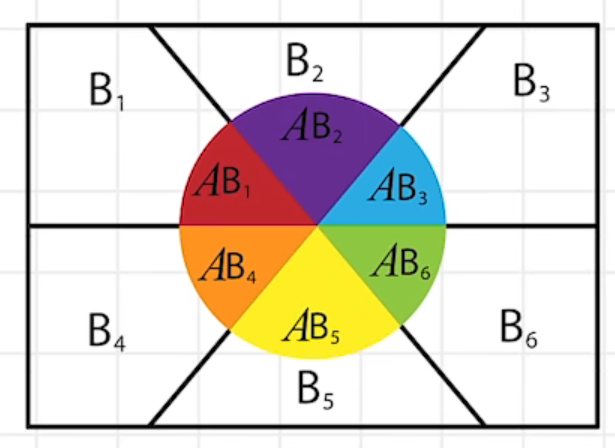
\includegraphics[width=0.3\textwidth,center]{../photo/quangailv.png}
\subsubsection{独立性}
\indent若事件$AB$独立,则$P(AB)=P(A)P(B),P(B)=P(B|A)=P(B|\overline{A})$。\\
\indent$A$和$B$互相独立,则$A$和$\overline{B}$,$\overline{A}$和$B$,$\overline{A}$和$\overline{B}$也互相独立。\\
\subsubsection{随机变量}
\indent对于随机变量$X$,称函数$F(X)=P(X\leq x)$为$X$的\textbf{分布函数},分布函数单调递增,$F(-\infty)=0,F(\infty)=1$。\\
\noindent\textbf{离散型随机变量}\\
\indent分布函数:$F(X)=\displaystyle\sum_{x_{k}\leq x}p_k$\\
\noindent\textbf{连续型随机变量}\\
\indent分布函数:$F(x)=\int_{-\infty}^{x}f(t)\text{d}t$,同样的$\int_{-\infty}^{\infty}f(t)\text{d}t=1$\\
\indent概率密度:$f(x)=F^{\prime}(x)$
\subsubsection{二项分布与泊松分布}
\indent二项分布:$P\{X=k\}=C_n^{k} p^{k} q^{n-k}(q=1-p)$\\
\indent泊松分布:$P\{X=k\}=\frac{\lambda^{k}e^{-\lambda}}{k!}$
\subsubsection{正态分布}
$X\sim N(\mu,\sigma^2)$其中$\mu$是期望,$\sigma^2$是方差。\\
\indent方差:$D(X)=E(X^2)-[E(x)]^2$。标准差$\sigma=\sqrt{D(x)}$
\subsubsection{期望}
\indent离散型随机变量的期望:$E(X)=\displaystyle\sum_{i=1}^{\infty}x_i p_i$\\
\indent连续型随机变量的期望:$E(X)=\int_{-\infty}^{\infty}xf(x)\text{d}x$\\
\indent$E(CX)=CE(X),E(X+Y)=E(X)+E(Y)$\\
\indent设$X,Y$互相独立,则$E(XY)=E(X)E(Y)$


\section{高精度算法}
\begin{lstlisting}[language=c++]
const int maxn = 1000;//maxn越大速度越慢
struct bign{
    int d[maxn], len;
    void clean() { while(len > 1 && !d[len-1]) len--; }
    bign() { memset(d, 0, sizeof(d)); len = 1; }
    bign(int num) { *this = num; } 
    bign(char* num) { *this = num; }
    bign operator = (const char* num){
        memset(d, 0, sizeof(d)); len = strlen(num);
        for(int i = 0; i < len; i++) d[i] = num[len-1-i] - '0';
        clean();
        return *this;
    }
    bign operator = (int num){
        char s[20]; sprintf(s, "%d", num);
        *this = s;
        return *this;
    }

    bign operator + (const bign& b){
        bign c = *this; int i;
        for (i = 0; i < b.len; i++){
            c.d[i] += b.d[i];
            if (c.d[i] > 9) c.d[i]%=10, c.d[i+1]++;
        }
        while (c.d[i] > 9) c.d[i++]%=10, c.d[i]++;
        c.len = max(len, b.len);
        if (c.d[i] && c.len <= i) c.len = i+1;
        return c;
    }
    bign operator - (const bign& b){
        bign c = *this; int i;
        for (i = 0; i < b.len; i++){
            c.d[i] -= b.d[i];
            if (c.d[i] < 0) c.d[i]+=10, c.d[i+1]--;
        }
        while (c.d[i] < 0) c.d[i++]+=10, c.d[i]--;
        c.clean();
        return c;
    }
    bign operator * (const bign& b)const{
        int i, j; bign c; c.len = len + b.len; 
        for(j = 0; j < b.len; j++) for(i = 0; i < len; i++) 
            c.d[i+j] += d[i] * b.d[j];
        for(i = 0; i < c.len-1; i++)
            c.d[i+1] += c.d[i]/10, c.d[i] %= 10;
        c.clean();
        return c;
    }
    bign operator / (const bign& b){
        int i, j;
        bign c = *this, a = 0;
        for (i = len - 1; i >= 0; i--)
        {
            a = a*10 + d[i];
            for (j = 0; j < 10; j++) if (a < b*(j+1)) break;
            c.d[i] = j;
            a = a - b*j;
        }
        c.clean();
        return c;
    }
    bign operator % (const bign& b){
        int i, j;
        bign a = 0;
        for (i = len - 1; i >= 0; i--)
        {
            a = a*10 + d[i];
            for (j = 0; j < 10; j++) if (a < b*(j+1)) break;
            a = a - b*j;
        }
        return a;
    }
    bign operator += (const bign& b){
        *this = *this + b;
        return *this;
    }

    bool operator <(const bign& b) const{
        if(len != b.len) return len < b.len;
        for(int i = len-1; i >= 0; i--)
            if(d[i] != b.d[i]) return d[i] < b.d[i];
        return false;
    }
    bool operator >(const bign& b) const{return b < *this;}
    bool operator<=(const bign& b) const{return !(b < *this);}
    bool operator>=(const bign& b) const{return !(*this < b);}
    bool operator!=(const bign& b) const{return b < *this || *this < b;}
    bool operator==(const bign& b) const{return !(b < *this) && !(b > *this);}

    string str() const{
        char s[maxn]={};
        for(int i = 0; i < len; i++) s[len-1-i] = d[i]+'0';
        return s;
    }
};
istream& operator >> (istream& in, bign& x)
{
    string s;
    in >> s;
    x = s.c_str();
    return in;
} 
ostream& operator << (ostream& out, const bign& x)
{
    out << x.str();
    return out;
}
int main()
{
    bign a, b;
    while (cin >> a >> b) cout << a+b << endl;
    return 0;
}
\end{lstlisting}
\ifx\allfiles\undefined
\end{document}
\fi
